\section{Dangermouse}

\margininbox{Dangermouse}{
     \begin{itemize}
    \item Jarvist Frost
    \item Paul Hutton
    \item Iztok Možir
    \end{itemize}}{\explo}

\begin{verse}
\note He's the greatest! He's Fantastic!\\
        Wherever there is danger he'll be there! \enote
\end{verse}


\tweet{2:53PM Aug 6, 2008}{M2:AJ/JH past 70s limit,tight rift.GW:JF/PH/IM new big pitch DANGERMOUSE off mudslump.Attempt at vocal con,no joy.Confluence at bot M2}

With a load of food and bolts, we shot down to \passage{Something Fishy} and dived down the right crawl. Drafting, with deep sand floor (all spoiled!). Became rather tight after $\approx$ 7 m.

So we hit the pitch, belay off jammed boulder, soon with a bolt.

Paul and Izi set off to grab the second bolt kit. Hopped down second pitch (6m) and came to something seemingly identical. Rigged off obvious natural and dropped down to choosy shelf $\approx$ 8 m. Then I turned around. Small pitch it was not. Boulders banged for 6s plus. Water could be heard a long way down, nothing visible (not even a drip!). The way to the \passage{M2} confluence?

From -25 m (limit), one could peer down past cascades into\ldots{} blackness. Big chamber?

Left $\approx$ 50 m of 10 mm at last bolt, PSS on sticking-out ledge + bolt kit and 2nd bolt kit at head of \passage{Something Fishy}. Early exit $\approx$ 1AM.

We blew trumpets every hour and listened every x 30 minutes - nothing from the \passage{M2} crew.

\name{Jarvist Frost}


\begin{survey}
\centering
\frame{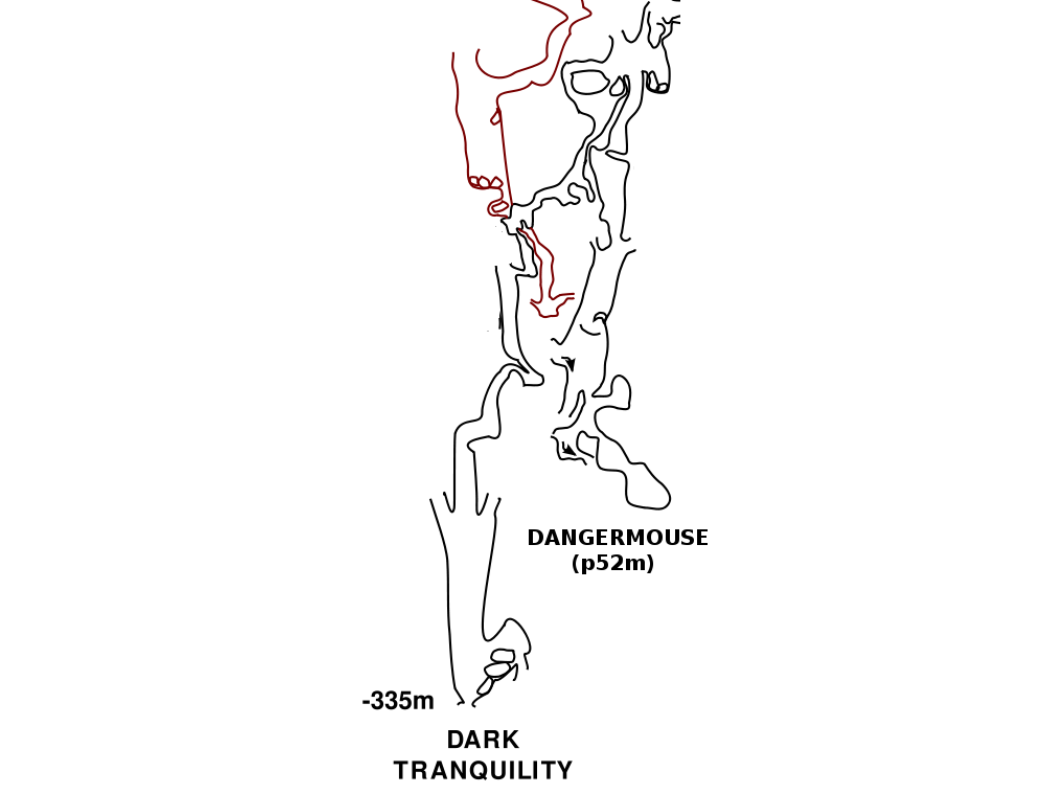
\includegraphics[width=\textwidth]{2008/dangermouse/dangermouse2_bcra_2008.pdf.png}}
\caption[Dangermouse]{Survey data of \passage{Dangermouse}, with pitches in \passage{M2} in red.}
\label{Dangermouse survey}
\end{survey}


\subsection{9th Aug - Dangermouse Continued}

\margininbox{Dangermouse}{
     \begin{itemize}
    \item Jarvist Frost
    \item Paul Hutton
    \item Martin McGowan
    \item Tim Osborne
    \end{itemize}}{\explo}


Despite being on several expeditions I have managed to always find somewhere else to go caving, but despite memories of Rik and Marcin's exploration of \passage{Captain Kangaroo} I was lulled into going down to
\passage{Dangermouse}. On the way down \passage{CK} it was noticeable that there is a certain lack of quality rigging - reminding me of the early \textit{Ben's Crap Lead}\sidenote{Former name of \passage{Vrtnarija}} rigging. \passage{Bonus Chamber} could do with a traverse line before you
swing out over the pitch. The near two sections of the cave,
\passage{Scrotty} and \passage{Even Scrottier}, again with a few hours of bashing and reshaping could change the passage to something nearer normal type passage.

    \begin{marginfigure}
\checkoddpage \ifoddpage \forcerectofloat \else \forceversofloat \fi
\centering
 \frame{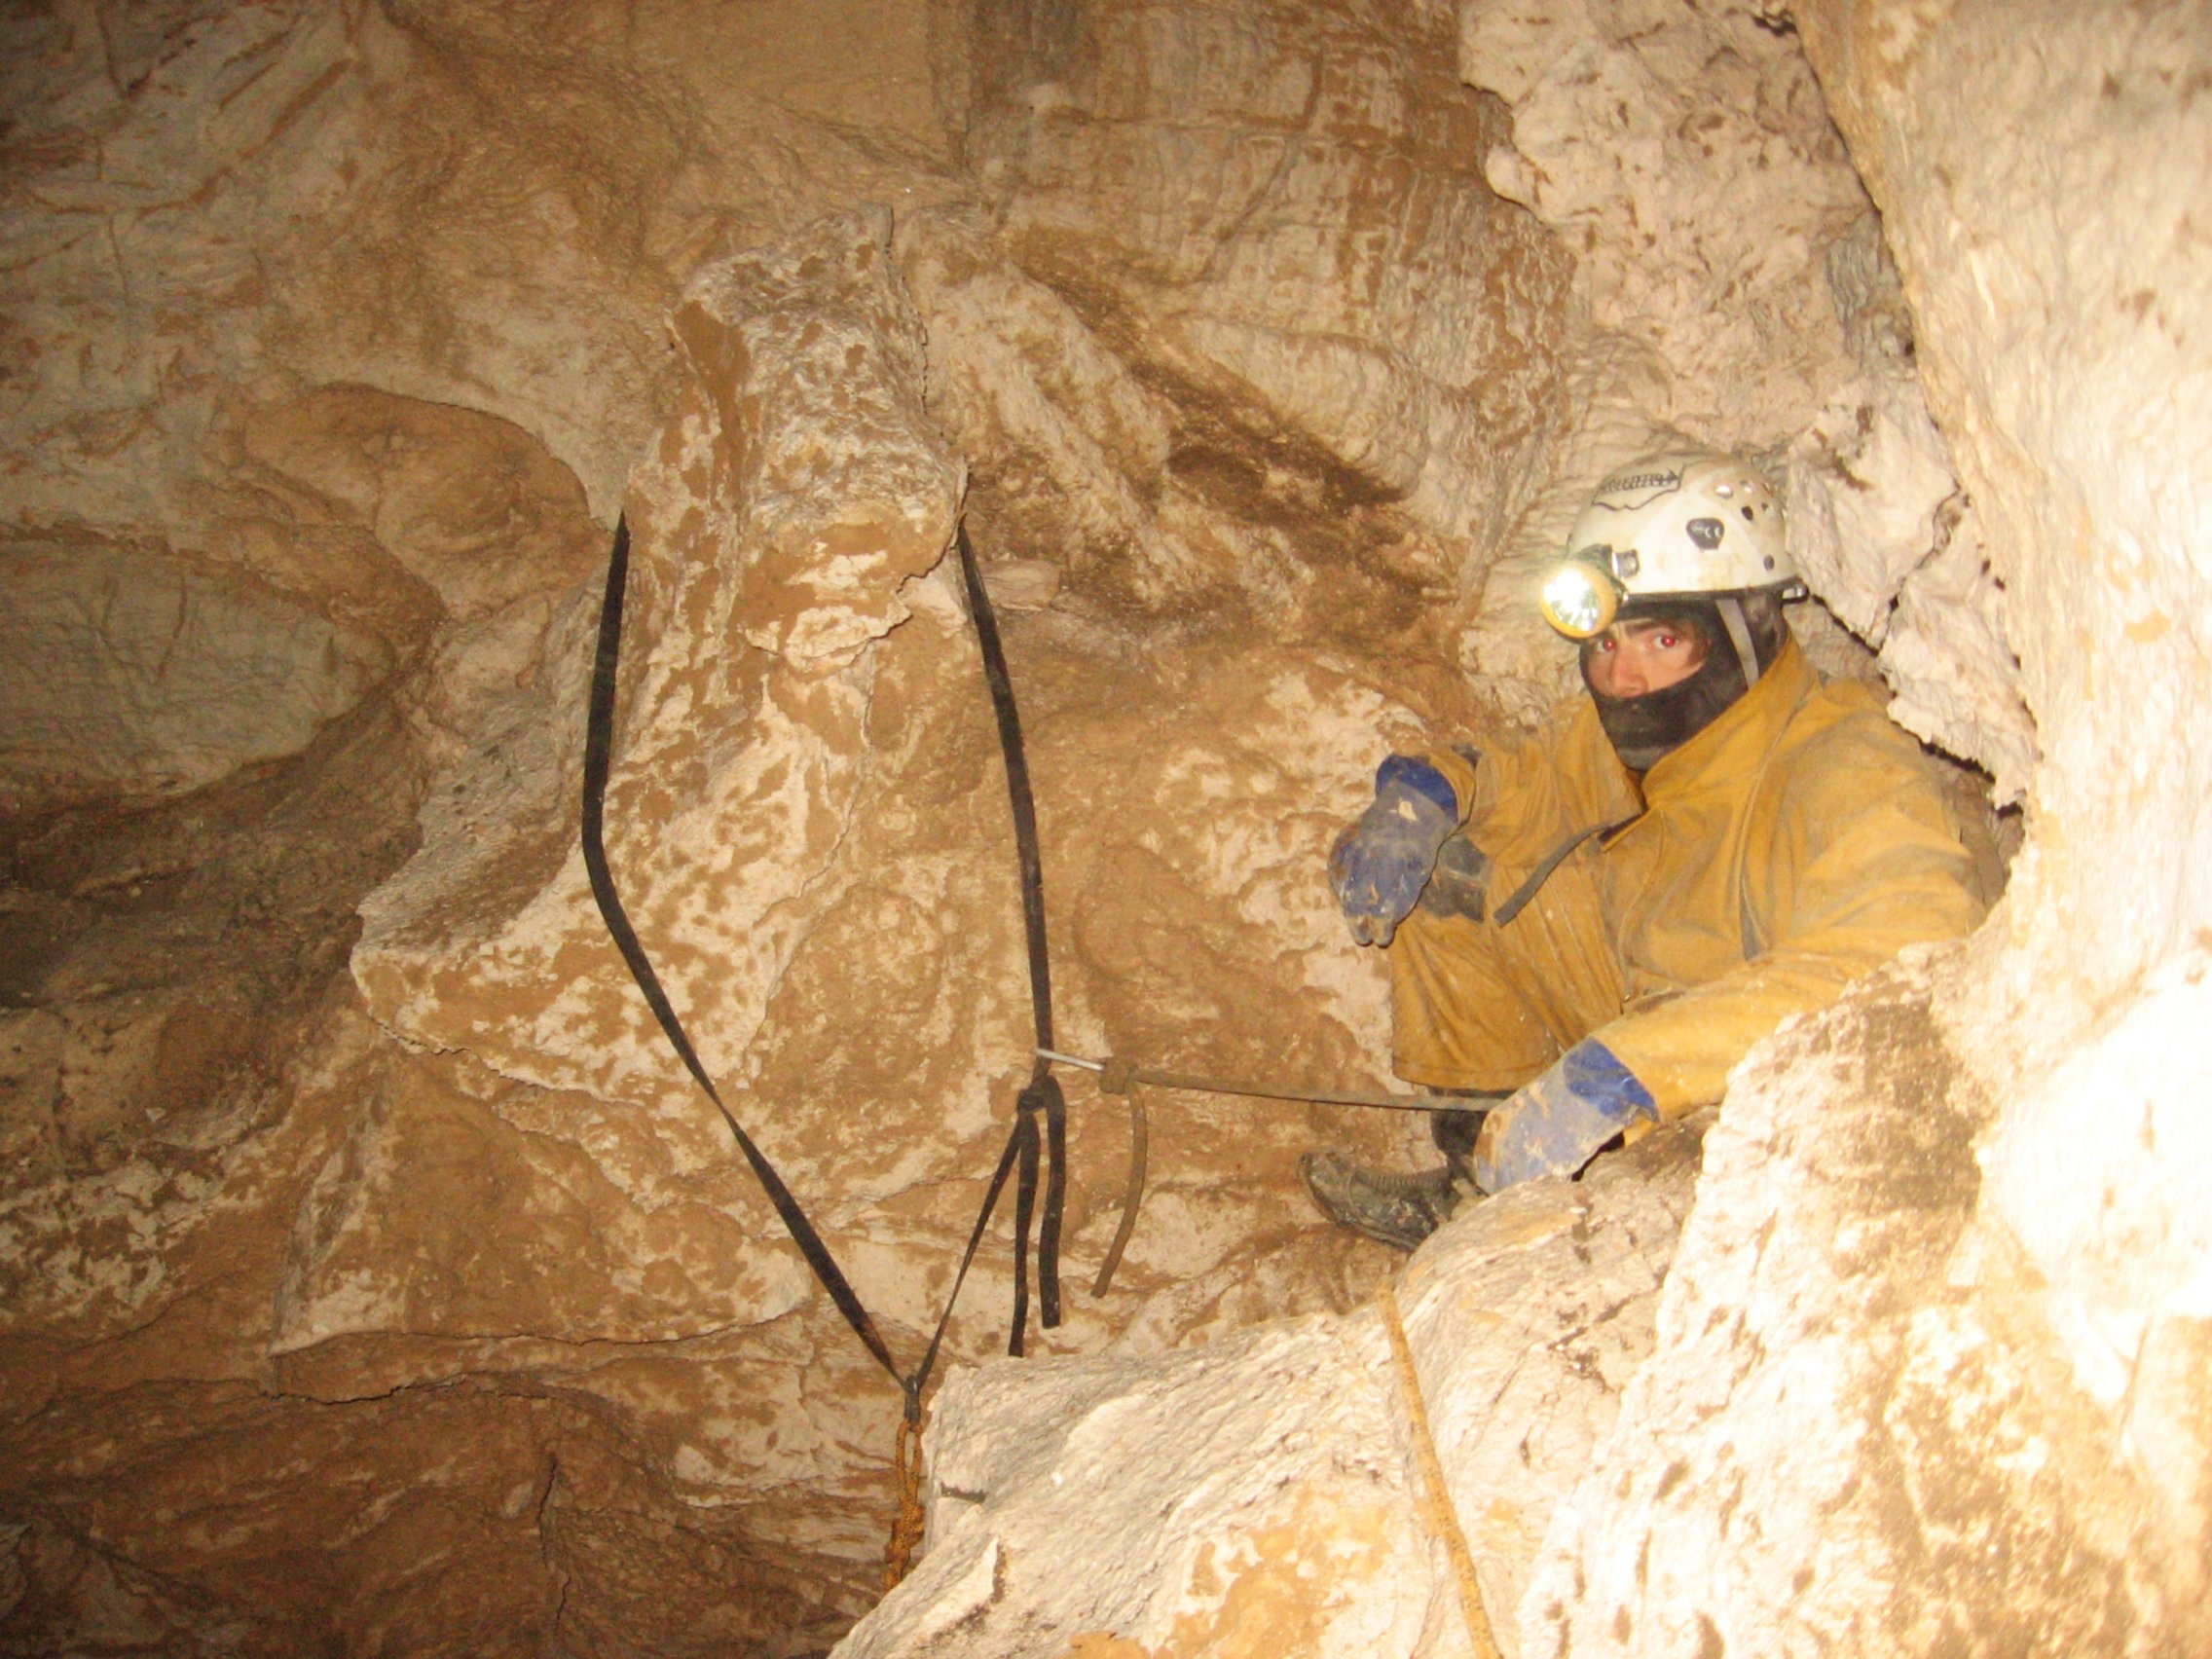
\includegraphics[width=\linewidth]{2008/dangermouse/Jarvist Frost - canon a520 -dangermouse - paul perched halfway down waiting for martin to bolt--orig.jpg}} 
 \caption{Paul waiting halfway down. \pic{Jarvist Frost}}
 \label{dangermouse}
\end{marginfigure}

At \passage{Dangermouse} I headed down to Jarv's bolt and set about clearing the pitch. Several large boulders were pushed down to a large resounding boom and crack of shattering rocks. From the first bolt I continued the gardening to a large natural in a corner. Paul followed on
down, and then Jarv. From the natural we descended via one bolt to a window. A small moment of disco leg occurred when a large chunk of the wall came off as I stood on it.

Paul came down to the window and took over the bolting. Eventually, after the first attempt broke the wall we had a bolt. I then sent / volunteered Paul to traverse over the pitch head to a possible rift / alcove. Unfortunately it turned out to be an alcove, so after a quick piss Paul returned, and went down the pitch to the bottom. He declared it dead and I followed as far as a ledge above, then Jarv went to the bottom for his compulsory photo op. Finally Tim joined us. While waiting on Jarv to finish his photography I started to throw stones down a small squeeze.

\begin{marginfigure}
\checkoddpage \ifoddpage \forcerectofloat \else \forceversofloat \fi
\centering
 \frame{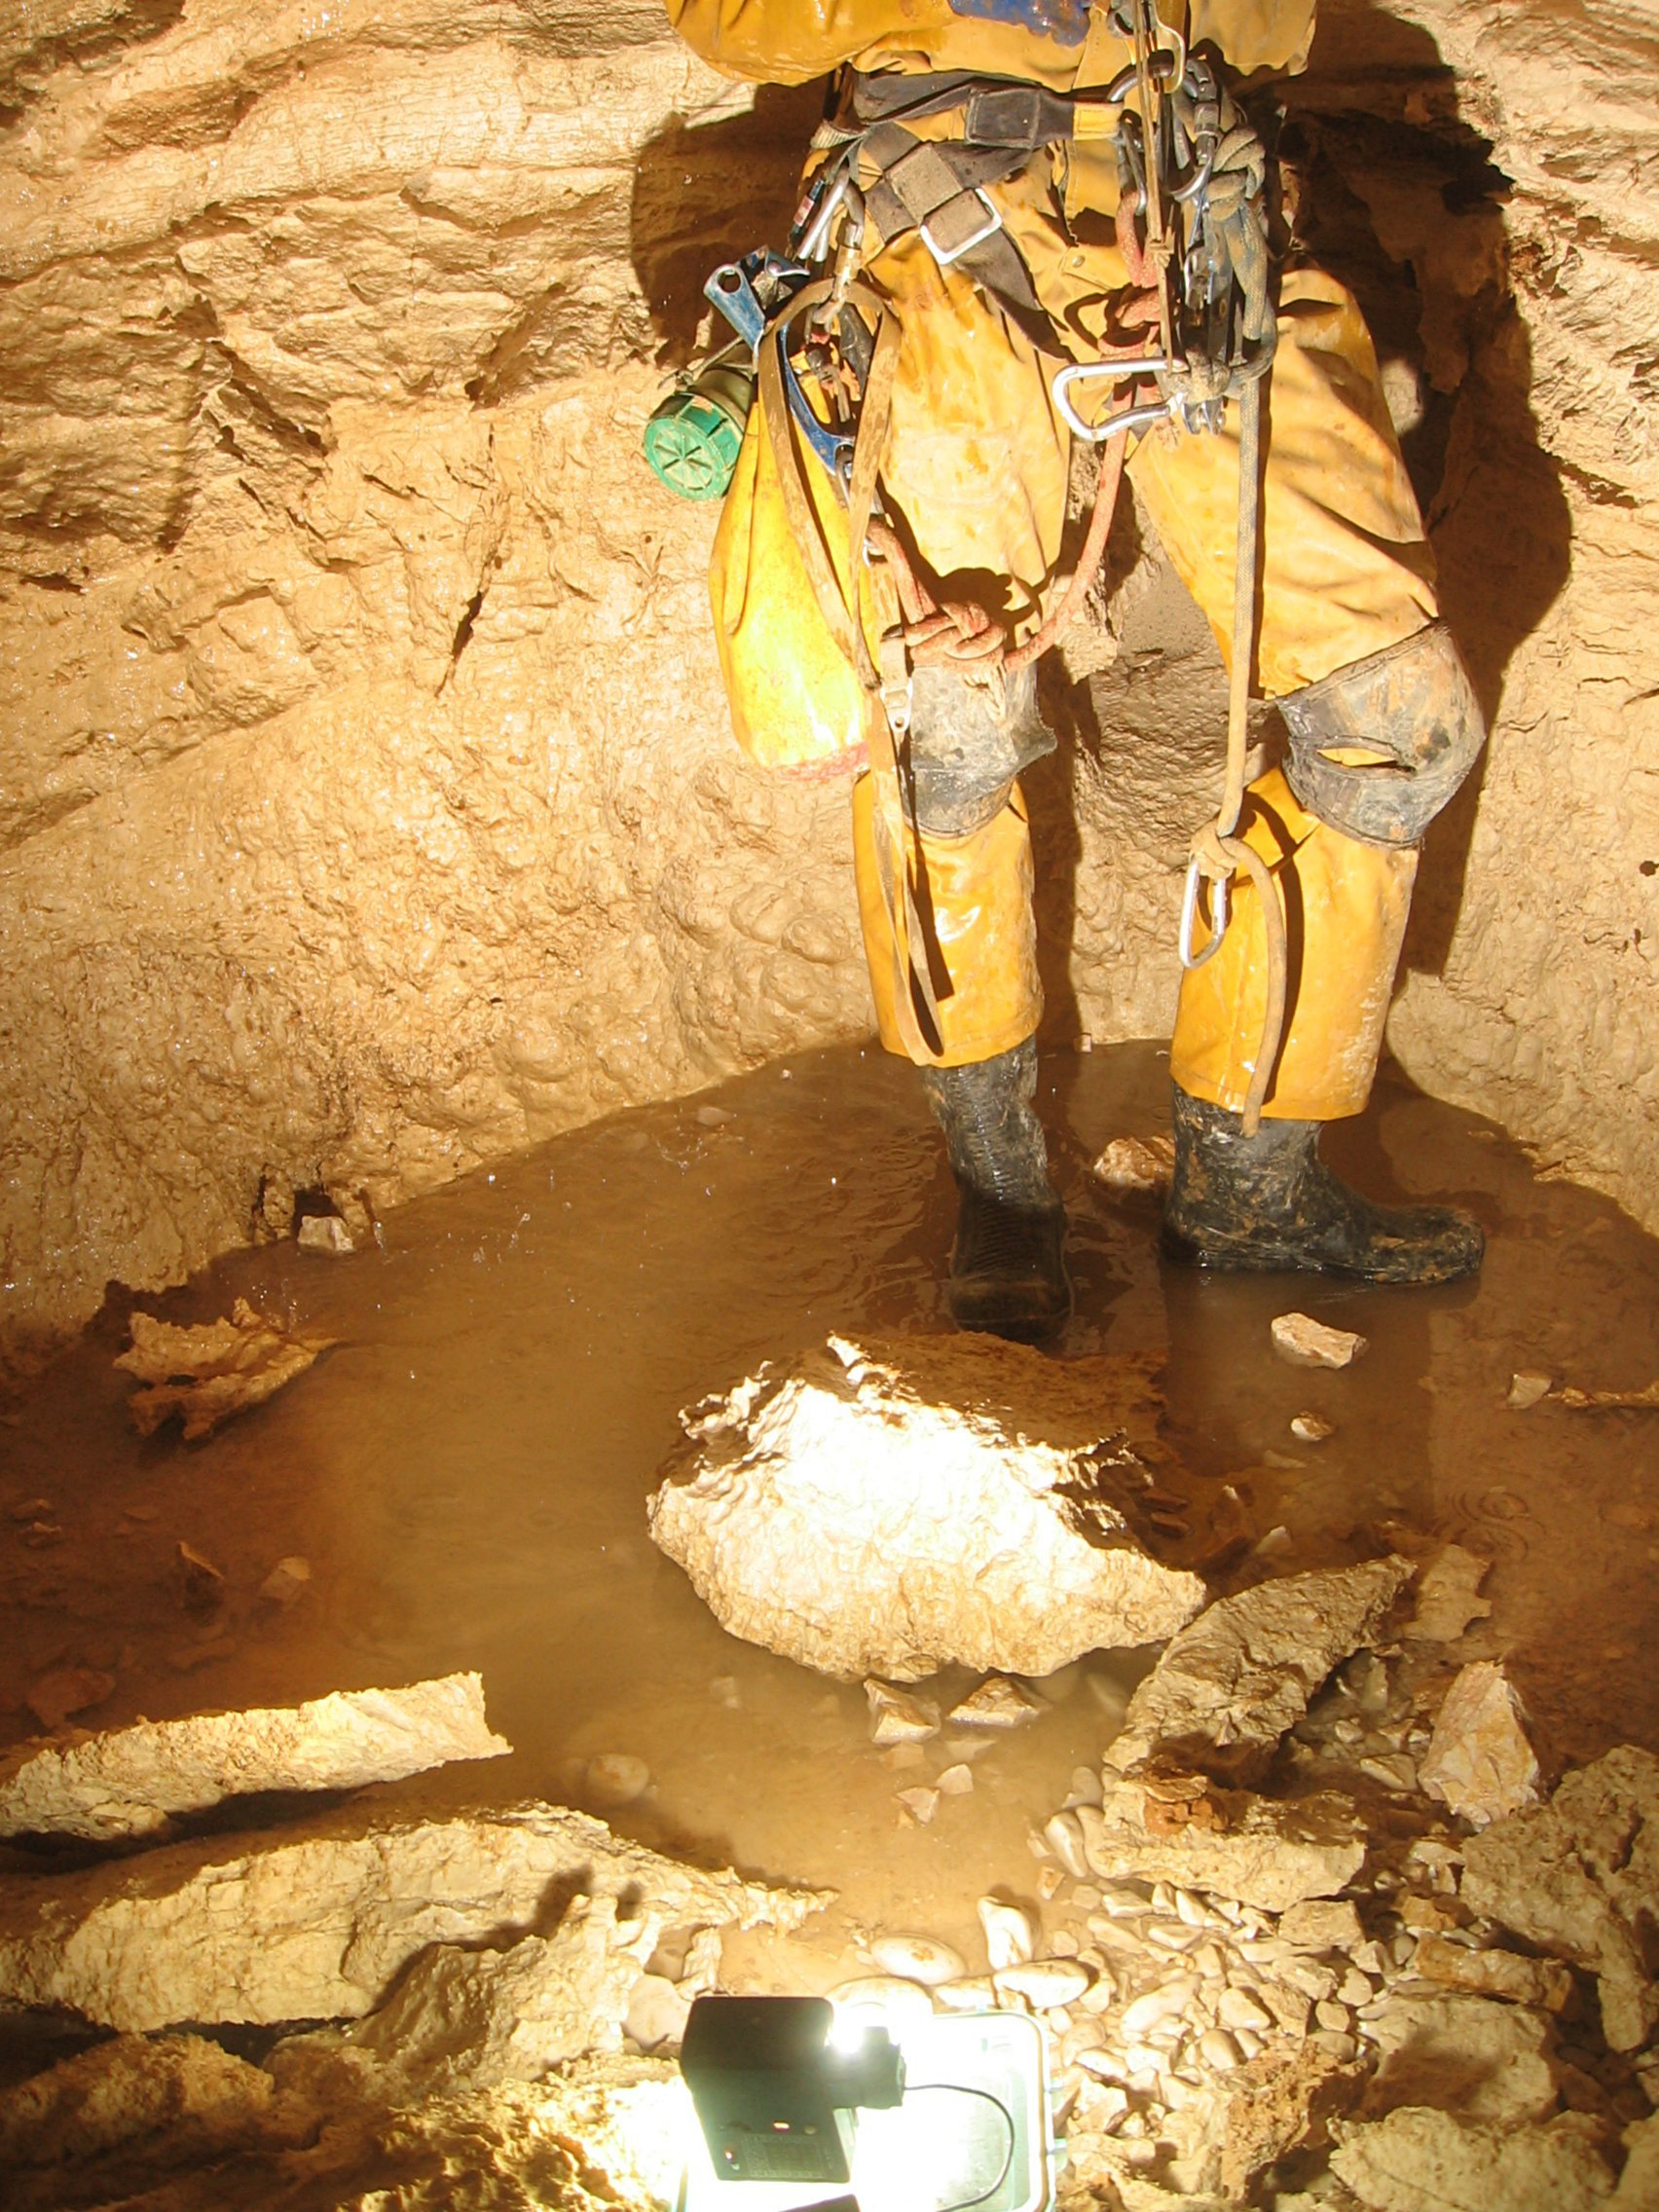
\includegraphics[width=\linewidth]{2008/dangermouse/Jarvist Frost - canon a520 -dangermouse - pool before exit streamway paul getting feet wet--orig.jpg}} 
 \caption{Paul standing in the small pool at the base of \passage{Dangermouse}. \pic{Jarvist Frost}}
 \label{dangermouse pool}
\end{marginfigure}

From beyond the squeeze a resounding boom could be heard. So quickly the rope was pulled up leaving Jarv and Paul stranded below and Tim went down. Unfortunately he faced the wrong way and could not turn his head to see down the pitch. Putting my stop on my cowstails I descended for a
quick look. After the squeeze the cave opens out into a chamber.

So while Paul and Jarv surveyed out Tim placed his first bolt and rigged the descent. A first for \passage{CK}, we backed up the descent: a figure of eight to a bolt and then an alpine butterfly onto a sling round a natural. All of this beautiful rigging was executed by Tim. So we made quick visit to the continuation and can confirm it is going somewhere.

Further Thoughts: We need a demolition team to visit \passage{Scrotty} and hammer, beat it into shape.

\name{Martin McGowan}


\tweet{1:25PM Aug 10th, 2008}{DANGERMOUSE bottomed and surveyed in at P52m. Mini streamway enters pitch, new P heads off after meander.}